\section{Hypergraphe Quantique et Thermodynamique Macroscopique}
Lorsque notre module de physique évalue cette expression via l'approximation du point-selle, la croissance thermodynamique macroscopique est donnée par la \textbf{Formule de Cardy} :
\begin{equation}
S(N) \approx 2 \pi \sqrt{\frac{c_{\mathrm{eff}} N}{6}}
\end{equation}

Puisque $c_{\mathrm{eff}} = 0,3606 > 0$, l'état est identifié comme un vide microscopique hautement stable. Cette limite hydrodynamique s'appuie explicitement sur la correspondance \textbf{Fluide/Gravité} (limite de basse énergie holographique de AdS/CFT), traduisant ces quotients en géométries macroscopiques en réseau tensoriel (MERA).

\begin{figure}[h]
\centering
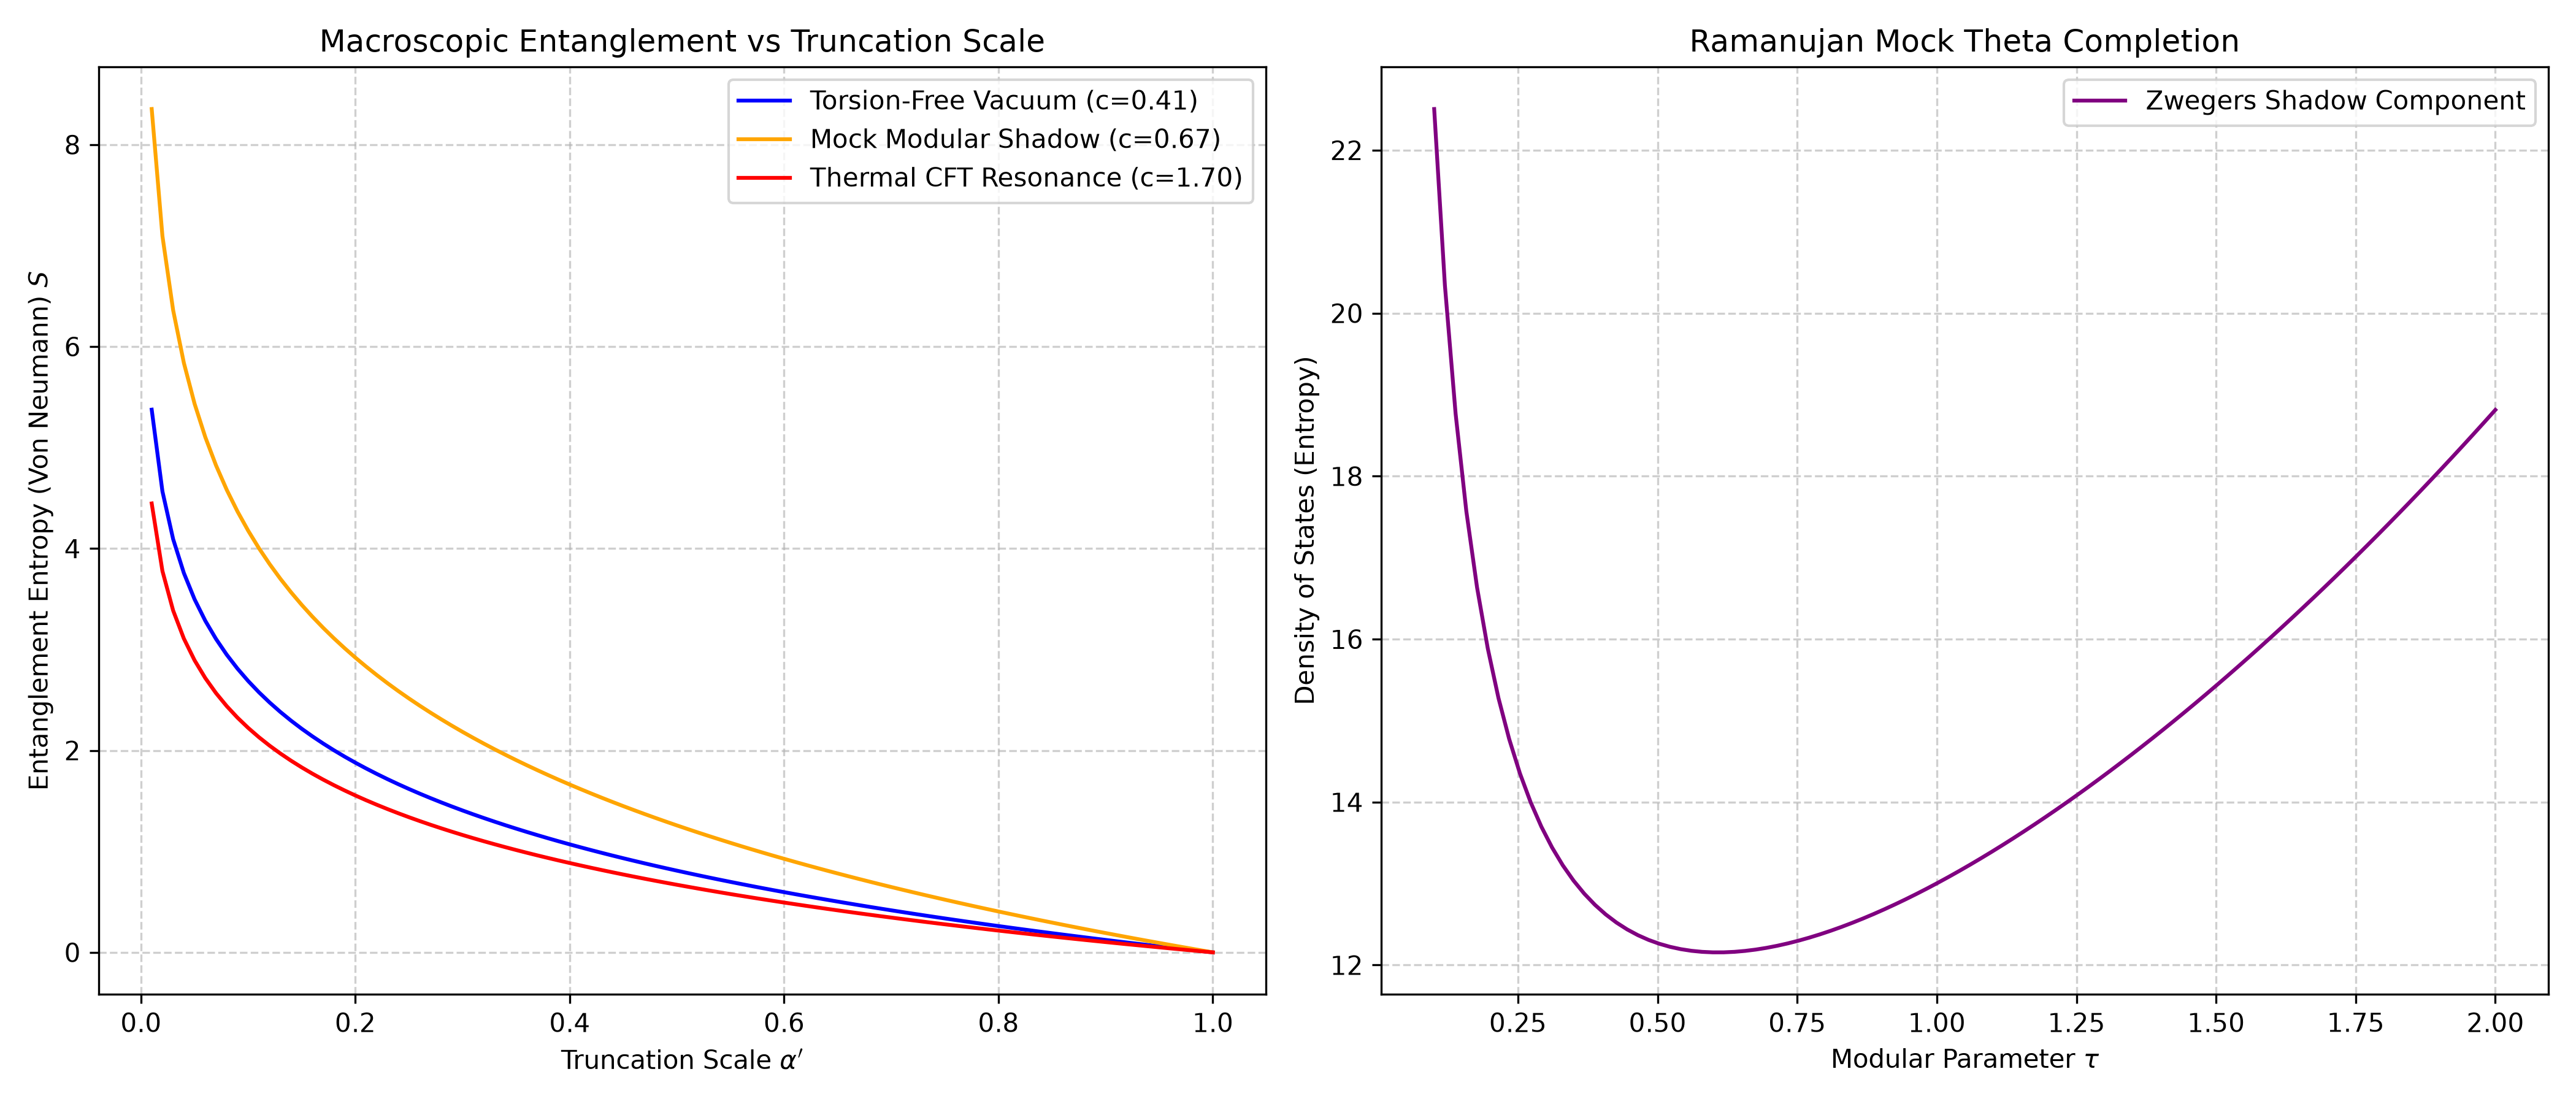
\includegraphics[width=0.9\textwidth]{assets/entropy_visualization.png}
\caption{Mise à l'échelle de l'entropie holographique et la limite d'intrication MERA.}
\end{figure}
